\documentclass[11pt,a4paper]{article}

\usepackage[utf8]{inputenc}
\usepackage[T1]{fontenc}
\usepackage[spanish,es-tabla,es-noshorthands]{babel} % noshorthands: que " no se convierta en diéresis
\usepackage[margin=2.5cm]{geometry}
\usepackage{booktabs}
\usepackage{enumitem}
\usepackage{graphicx}
\usepackage{float} % [H]: la figura va justo donde se escribe
\usepackage{amsmath}
\usepackage{amssymb}
\usepackage[hidelinks]{hyperref}

\setlist{nosep}
\setlength{\parskip}{0.5em}
\setlength{\parindent}{0pt}
\setlength{\emergencystretch}{2em} % evita que el código largo se salga del margen

% Código en línea: \code{Folder.Files}. Los guiones bajos se escriben \_
\newcommand{\code}[1]{\texttt{#1}}
% Hueco para lo que falta por escribir
\newcommand{\pendiente}{\textit{Pendiente.}}

\title{Práctica 2: Visualización y análisis de datos con Power BI\\
\large Decisiones tomadas en cada ejercicio}
\author{Grupo 4: Iván y Álvaro}
\date{\today}

\begin{document}

\maketitle

\section*{Preparación de la gold}
Antes de conectar Power BI se han hecho dos cambios en la exportación de la Práctica 1:
\begin{itemize}
    \item \textbf{\code{coalesce(1)}:} cada tabla se exporta en un único fichero \code{.parquet}, así Power BI combina un solo fichero por tabla. Concentrar los datos en una partición sería un cuello de botella con volúmenes grandes, pero la gold ocupa alrededor de 1\,MB.
    \item \textbf{\code{Dia\_Semana\_Num} en \code{dim\_fecha}} (1 = lunes \ldots{} 5 = viernes): Power BI ordena el texto alfabéticamente (\textit{Friday}, \textit{Monday}\ldots), y esta columna permite ordenar \code{Dia\_Semana} con \textit{Ordenar por columna}.
\end{itemize}

\subsection*{Ej1: conectar e importar}
\begin{itemize}
    \item \textbf{Función:} conector \textit{Carpeta}, una vez por tabla (\code{hecho\_cotizacion}, \code{dim\_empresa}, \code{dim\_sector} y \code{dim\_fecha}), abriendo \textit{Transformar datos} para preparar cada consulta en Power Query.
    \item \textbf{Pasos en cada consulta:}
    \begin{enumerate}
        \item Filtro en \code{Extension} para quedarse solo con \code{.parquet}: Spark escribe además \code{\_SUCCESS} y ficheros \code{.crc}, que no son datos.
        \item \textit{Combinar archivos} sobre \code{Content}, que lee el Parquet y lo convierte en tabla.
        \item Quitar \code{Source.Name}, el nombre del fichero de origen, que no aporta nada.
        \item Revisar tipos: \code{Date} como fecha, \code{Volume}, \code{MarketCap}, \code{Anio}, \code{Mes}, \code{Trimestre} y \code{Dia\_Semana\_Num} como enteros, los precios, porcentajes y \code{Stock\_Splits} como decimales y el resto como texto.
        \item Renombrar la consulta: \code{hechos}, \code{dim\_empresa}, \code{dim\_sector} y \code{dim\_fecha}.
    \end{enumerate}
    \item \textbf{Resultado:} cuatro tablas en modo \textit{Import} (Power BI copia los datos a su modelo en memoria): \code{hechos} con 19\,152 filas, \code{dim\_empresa} con 36, \code{dim\_sector} con 11 y \code{dim\_fecha} con 532.
\end{itemize}

\subsection*{Ej2: modelo en estrella}
\begin{figure}[H]
    \centering
    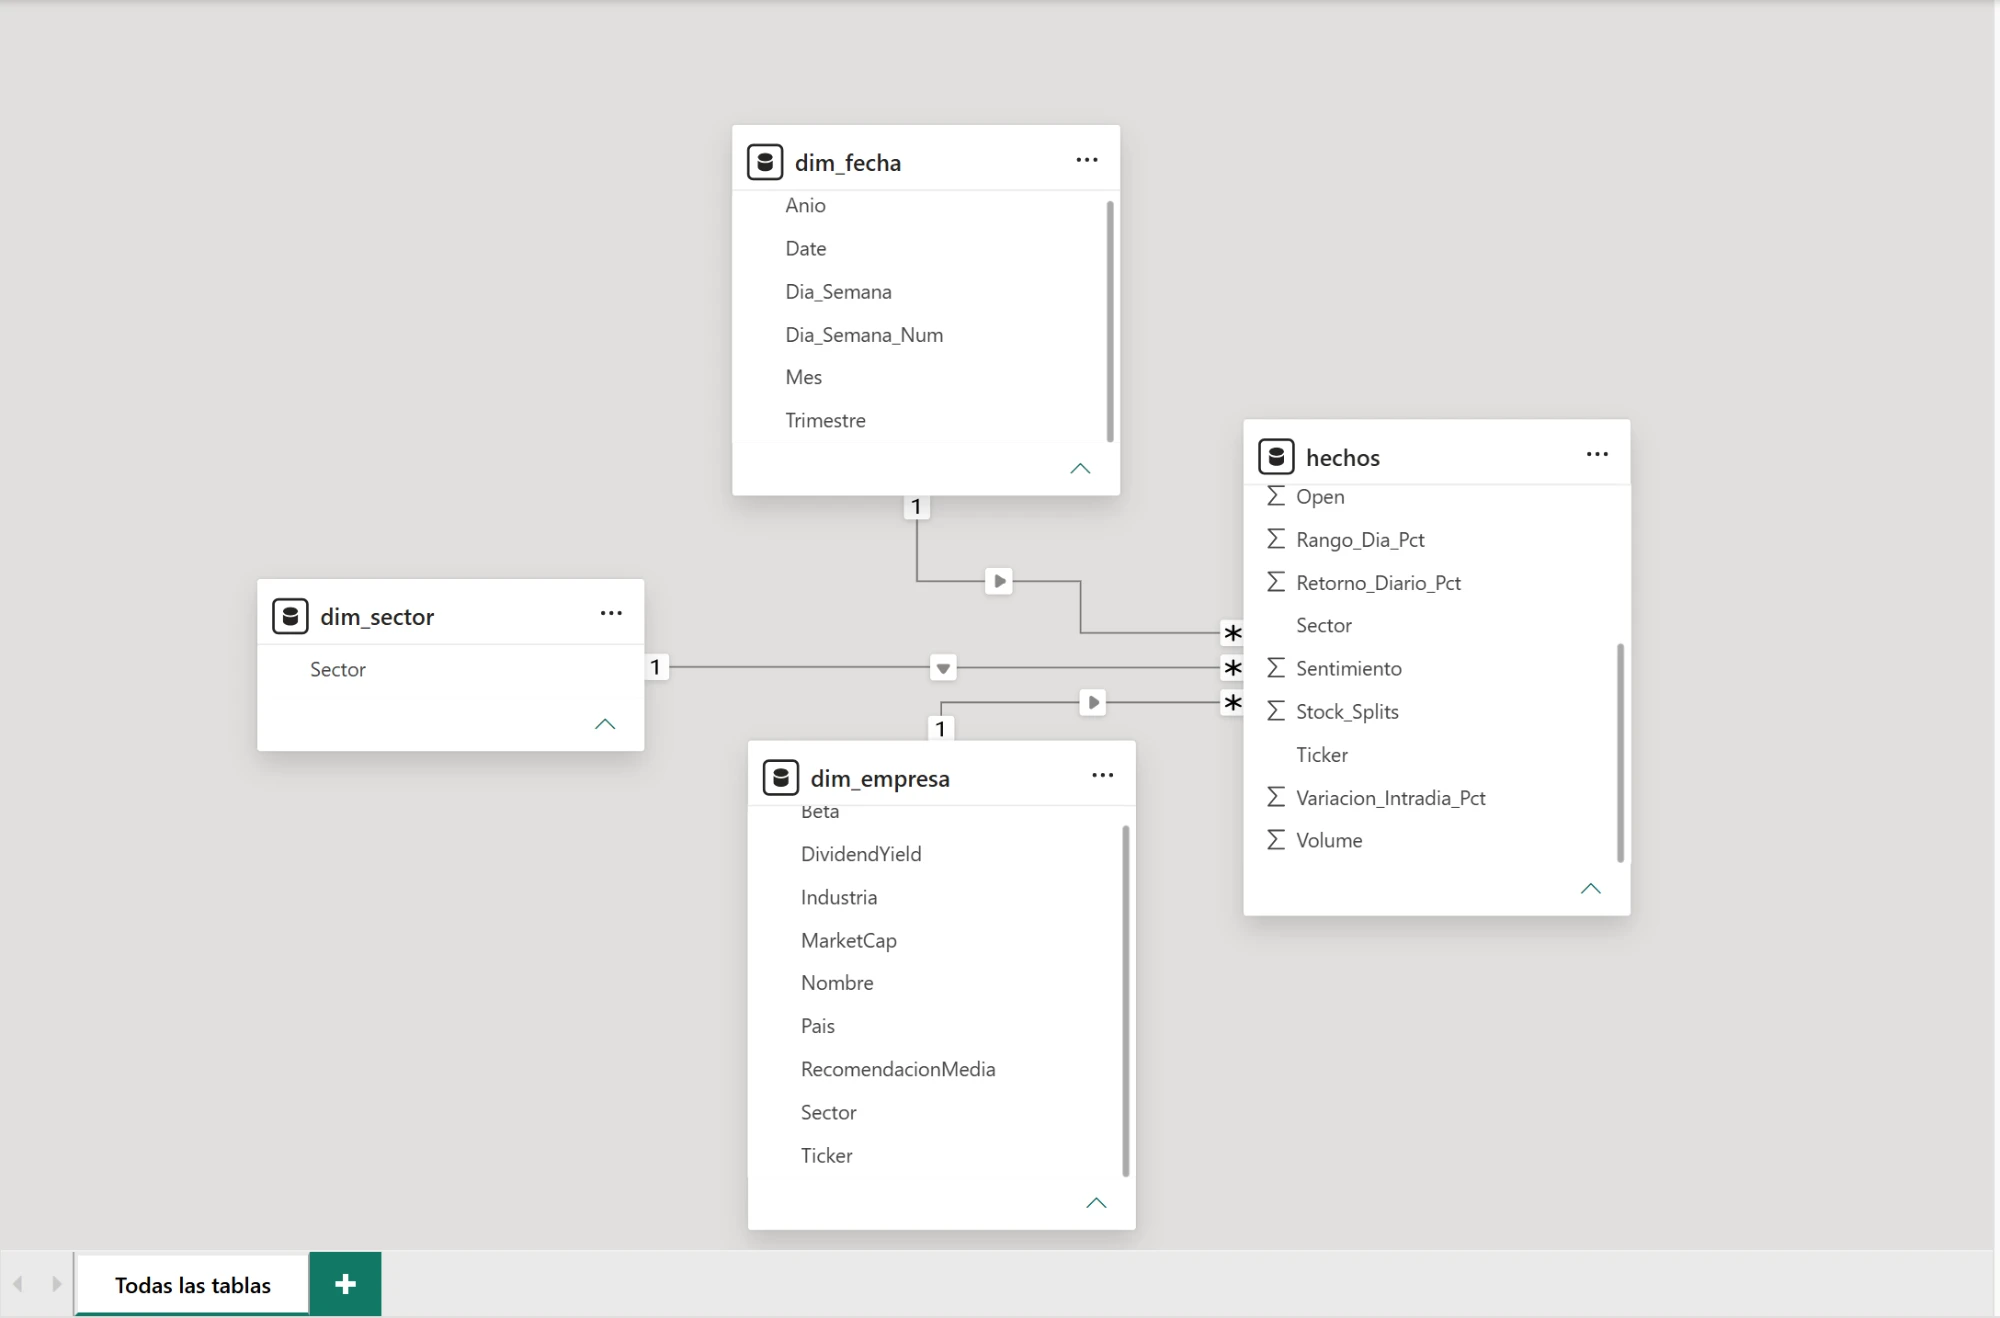
\includegraphics[width=0.85\textwidth]{img/modelo_estrella.png}
    \caption{Modelo en estrella en la vista Modelo de Power BI.}
\end{figure}
\begin{itemize}
    \item \textbf{Diseño relacional y granularidad:} se implementa un \textbf{Modelo en Estrella puro} (\textit{Star Schema}) bajo los principios de diseño dimensional de Ralph Kimball. La tabla central \code{hechos} concentra las métricas cuantitativas periódicas de cotización a nivel de grano \code{(Ticker, Date)} (19\,152 filas). Alrededor orbitan tres tablas de dimensiones puras que aportan el contexto descriptivo: temporal (\code{dim\_fecha}), empresarial (\code{dim\_empresa}) y de clasificación macroeconómica (\code{dim\_sector}).
    \item \textbf{Relaciones activas del modelo (líneas continuas):}
    \begin{itemize}
        \item \textbf{\code{dim\_fecha[Date]} $\mathbf{(1) \longrightarrow (*)}$ \code{hechos[Date]}:} relación uno a varios activa con filtrado unidireccional (\textit{Single}). Permite filtrar la serie temporal por jerarquías de calendario (\code{Anio}, \code{Trimestre}, \code{Mes}, \code{Dia\_Semana}). Cada fecha única en la dimensión se asocia a las 36 cotizaciones simultáneas de esa sesión en \code{hechos}.
        \item \textbf{\code{dim\_empresa[Ticker]} $\mathbf{(1) \longrightarrow (*)}$ \code{hechos[Ticker]}:} relación uno a varios activa con filtrado unidireccional. Asocia cada sesión a los atributos corporativos estáticos (\code{Nombre}, \code{Industria}, \code{MarketCap}, \code{Beta}, \code{DividendYield}). Cada empresa única se vincula a sus ~532 sesiones registradas.
        \item \textbf{\code{dim\_sector[Sector]} $\mathbf{(1) \longrightarrow (*)}$ \code{hechos[Sector]}:} relación uno a varios activa con filtrado unidireccional. Permite realizar agrupaciones y agregaciones sectoriales (retorno medio por sector, sentimiento medio del analista, volatilidad sectorial) de forma directa e inmediata sobre las métricas de cotización.
    \end{itemize}
    \item \textbf{Justificación de la relación inactiva (\code{dim\_sector} $\mathbf{\dashrightarrow}$ \code{dim\_empresa}):} durante la importación, Power BI detecta automáticamente la columna homónima \code{Sector} presente tanto en \code{dim\_empresa} como en \code{dim\_sector} e intenta crear un vínculo relacional entre ellas. Si dicha relación se mantuviese activa simultáneamente con las demás, se incurriría en dos problemas de arquitectura relacional:
    \begin{enumerate}
        \item \textbf{Rutas de filtrado ambiguas y cíclicas:} existirían dos caminos concurrentes para que el filtro de sector alcance la tabla de hechos:
        \[ \text{Ruta directa: } \code{dim\_sector} \longrightarrow \code{hechos} \]
        \[ \text{Ruta indirecta: } \code{dim\_sector} \longrightarrow \code{dim\_empresa} \longrightarrow \code{hechos} \]
        Esta redundancia genera ambigüedad semántica en el motor analítico VertiPaq, obligando a Power BI a desactivar una de las dos vías o arriesgarse a evaluaciones inconsistentes del contexto de filtro en medidas DAX complejas.
        \item \textbf{Degradación a Copo de Nieve (\textit{Snowflake Schema}):} activar la relación indirecta normalizaría las dimensiones, convirtiendo el diseño en un copo de nieve. La literatura de BI y las directrices de Kimball desaconsejan este esquema salvo casos de cardinalidad extrema, ya que añade saltos de \textit{join} adicionales, ralentiza el escaneo columnar en memoria y complica la comprensión del modelo para los autores de informes.
    \end{enumerate}
    Por tanto, mantener esta relación deliberadamente \textbf{inactiva} (mostrada con línea punteada en la vista Modelo) es la decisión técnica correcta: asegura un estrella puro, elimina cualquier ambigüedad de contexto y maximiza la velocidad de cálculo. Si en un cálculo avanzado se requiriese propagar el filtro sectorial exclusivamente sobre atributos de \code{dim\_empresa}, DAX permite activarla de forma puntual mediante la función \code{USERELATIONSHIP(dim\_sector[Sector], dim\_empresa[Sector])}.
    \item \textbf{Dirección de filtro único y configuración de fechas:} todas las relaciones activas tienen dirección de filtro único (\textit{Single}), propagándose siempre desde la dimensión (lado 1) hacia la tabla de hechos (lado *). No se utiliza filtrado bidireccional (\textit{Both}), evitando bloqueos de rendimiento o propagaciones indeseadas. Asimismo, se ha deshabilitado la opción global de \textit{Fecha/hora automática} de Power BI, evitando la proliferación oculta de tablas de calendario locales y garantizando que el eje temporal responda exclusivamente a \code{dim\_fecha}.
\end{itemize}

\subsection*{Ej3: panorama}
\begin{figure}[H]
    \centering
    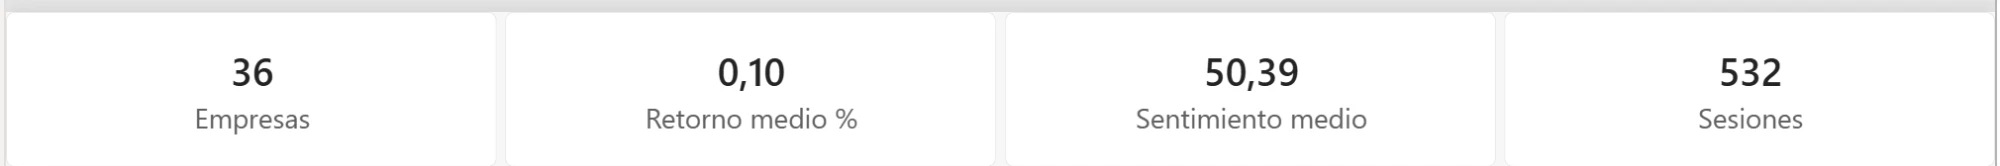
\includegraphics[width=\textwidth]{img/ej3_tarjeta.png}
    \caption{Tarjeta con las cuatro medidas del panorama.}
\end{figure}
\begin{itemize}
    \item \textbf{Gráfico:} un visual \textit{Tarjeta} con cuatro medidas en fila en la parte superior de la página. Una tarjeta destaca un único número que se lee de un vistazo, y es la cabecera natural del dashboard: da el contexto antes de entrar en los gráficos.
    \item \textbf{Medidas} (DAX, creadas en \code{hechos}):
    \begin{itemize}
        \item \code{Empresas = DISTINCTCOUNT(hechos[Ticker])}: empresas distintas; \code{COUNT} contaría filas (19\,152).
        \item \code{Sesiones = DISTINCTCOUNT(hechos[Date])}: días de cotización distintos.
        \item \code{Retorno medio \% = AVERAGE(hechos[Retorno\_Diario\_Pct])}: media del retorno diario.
        \item \code{Sentimiento medio = AVERAGE(hechos[Sentimiento])}: media del sentimiento del sector.
    \end{itemize}
    Se usan medidas explícitas en lugar de arrastrar las columnas porque las columnas numéricas se resumen por \textit{Suma} por defecto (la suma de los retornos no tiene sentido), y porque se definen una vez con su nombre y formato y se reutilizan en los ejercicios siguientes. \code{AVERAGE} ignora los nulos: el primer retorno de cada empresa y los días sin sentimiento.
    \item \textbf{Resultado:} 36 empresas, 532 sesiones, retorno medio de 0,10\,\% diario y sentimiento medio de 50,39. Los valores coinciden con los calculados en Spark sobre la misma gold.
    \item \textbf{Análisis:} el retorno medio diario es pequeño pero positivo, lo que en dos años supone una tendencia alcista del conjunto. El sentimiento medio queda prácticamente en el punto neutro (50). Como son medidas, se recalculan con los filtros que les lleguen; en el Ej4 se evita que el segmentador de empresa filtre la tarjeta para que siga mostrando el conjunto del IBEX.
\end{itemize}

\subsection*{Ej4: evolución del precio}
\begin{itemize}
    \item \textbf{Gráfico:} de líneas, porque muestra cómo evoluciona una magnitud a lo largo del tiempo y deja ver la tendencia, el ritmo del cambio y los puntos de giro.
    \item \textbf{Datos:} eje X \code{dim\_fecha[Date]} y eje Y \code{hechos[Close]} agregado como \textit{Promedio}. La fecha se toma de la dimensión para que el filtro viaje por la relación del modelo. Como se desactivó la fecha automática, el eje es continuo y sin jerarquía año/trimestre/mes.
    \item \textbf{Segmentador:} \code{dim\_empresa[Ticker]} en formato desplegable y con selección única. Con varias empresas (o ninguna, que equivale a todas) cada punto sería la media de precios de acciones muy distintas, una cifra que no es el precio de ninguna y que dominaría la más cara. Con selección única la línea es siempre el precio de cierre de una empresa.
    \item \textbf{Interacciones:} con \textit{Editar interacciones} el segmentador filtra solo el gráfico y no la tarjeta del Ej3, que mantiene el panorama del IBEX completo; con una empresa fija, \textit{Empresas} valdría siempre 1.
    \item \textbf{Línea de tendencia} (pestaña \textit{Análisis}): recta de regresión del precio frente al tiempo, que resume hacia dónde va la serie por encima del ruido diario.
\end{itemize}

\textbf{Análisis.} Se comentan tres empresas con comportamientos distintos, elegidas calculando en Spark la variación del cierre entre el 01-10-2024 y el 30-10-2026:
\begin{itemize}
    \item \textbf{Indra (\code{IDR.MC}), alcista:} pasa de 16,48\,€ a 63,88\,€ (+287,6\,\%), la mayor subida del índice. Tras unos meses planos, el salto empieza a finales de febrero de 2025 y la subida se mantiene, con correcciones, hasta máximos cerca de 65\,€. La serie se ajusta bien a la línea de tendencia.
    \item \textbf{Telefónica (\code{TEF.MC}), bajista:} pasa de 4,39\,€ a 3,37\,€ ($-$23,2\,\%), la mayor caída. Llega a un máximo de 4,89\,€ en septiembre de 2025, pero entre octubre y noviembre de 2025 cae de golpe de unos 4,6\,€ a menos de 3,7\,€ y no vuelve a acercarse a esos niveles.
    \item \textbf{Merlin (\code{MRL.MC}), lateral:} pasa de 11,35\,€ a 11,47\,€ (+1,1\,\%), pero entre medias sube de 8,61\,€ a 15,75\,€ y lo devuelve todo desde julio de 2026. Aquí la línea de tendencia sale alcista aunque el precio termina donde empezó: la regresión resume la serie con una recta y no capta un cambio de dirección. La tendencia hay que leerla junto con la propia línea.
\end{itemize}
\begin{figure}[H]
    \centering
    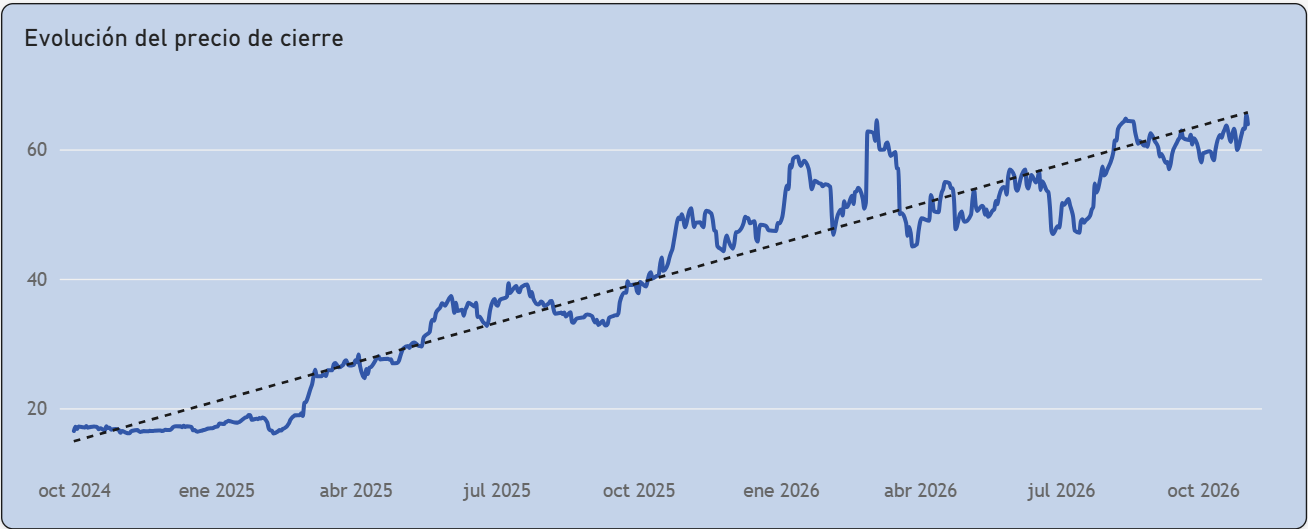
\includegraphics[width=\textwidth]{img/ej4_idr.png}\\[0.5em]
    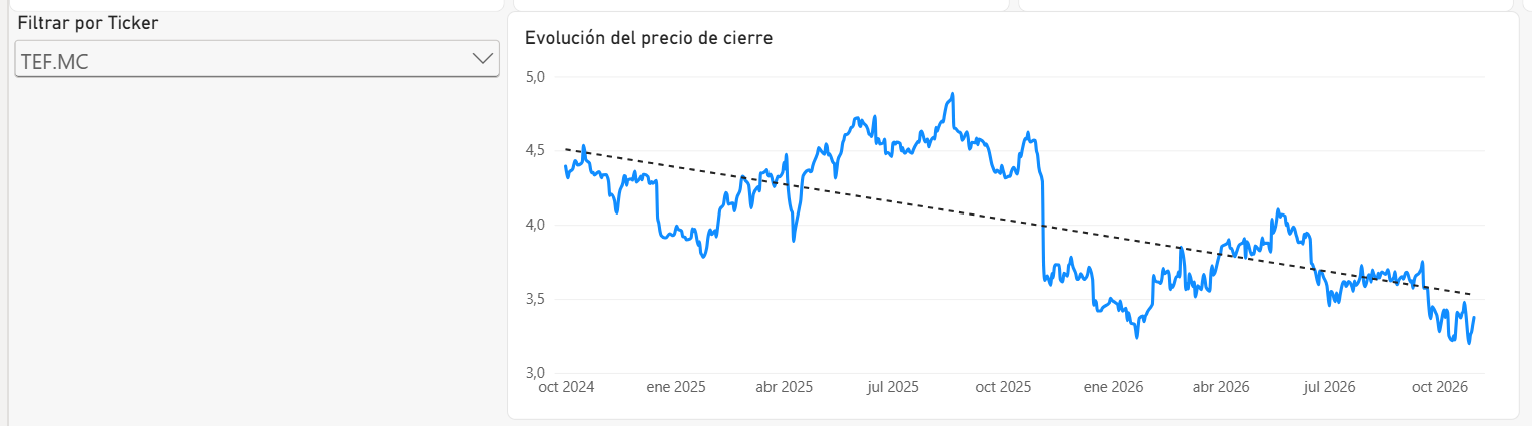
\includegraphics[width=\textwidth]{img/ej4_tef.png}\\[0.5em]
    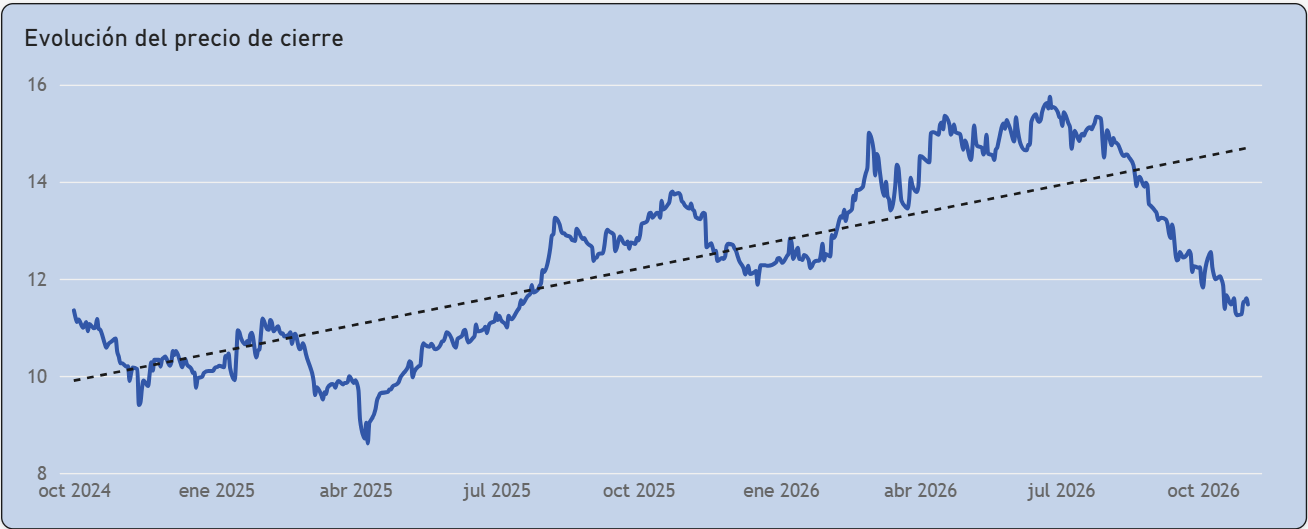
\includegraphics[width=\textwidth]{img/ej4_mrl.png}
    \caption{Evolución del precio de cierre de Indra, Telefónica y Merlin, con su línea de tendencia.}
\end{figure}

\subsection*{Ej5 (opcional): efecto viernes}
\begin{figure}[H]
    \centering
    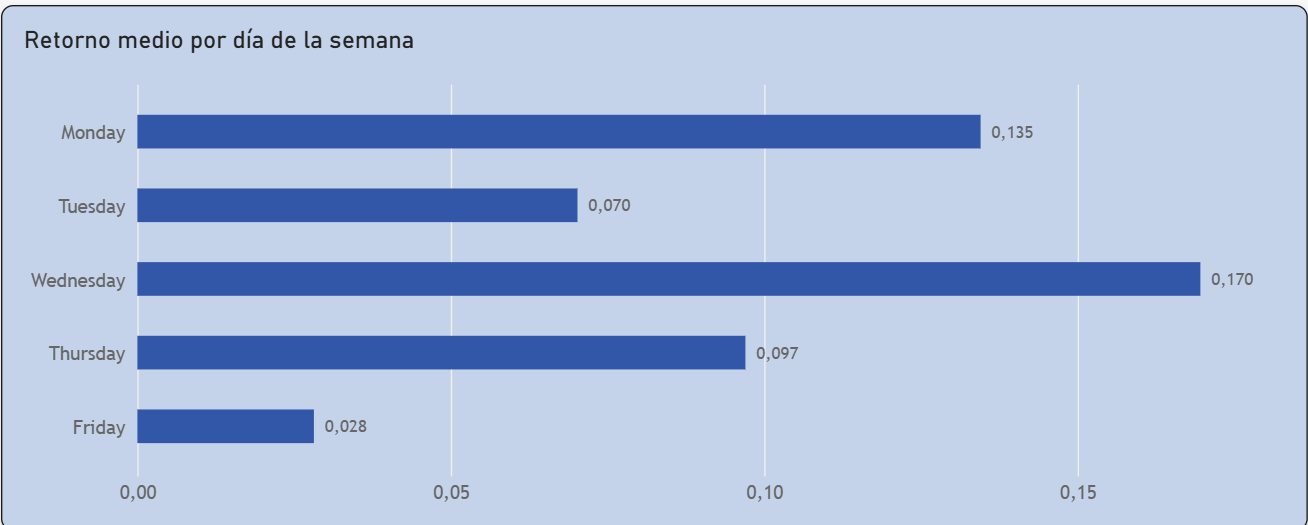
\includegraphics[width=0.55\textwidth]{img/ej5_viernes.png}
    \caption{Retorno medio por día de la semana.}
\end{figure}
\begin{itemize}
    \item \textbf{Gráfico:} de barras, porque compara una medida entre categorías, los cinco días de la semana. Los días se ordenan con \code{Dia\_Semana\_Num} para que vayan de lunes a viernes y no por orden alfabético.
    \item \textbf{Datos:} \code{dim\_fecha[Dia\_Semana]} y la medida \textit{Retorno medio \%} del Ej3. El segmentador de empresa no filtra este gráfico, así que muestra el mercado completo.
    \item \textbf{Análisis:} el viernes es el peor día, con 0,028\,\%, frente a 0,070--0,170\,\% del resto; el miércoles y el lunes son los mejores. El efecto viernes de las finanzas conductuales predice lo contrario, que los viernes suben más por el optimismo antes del fin de semana, así que en estos datos no se cumple. Aun así, las diferencias son de centésimas de punto y cada día suma unas 105 sesiones, por lo que unos pocos días extremos, como las caídas de abril de 2025, bastan para mover una barra. Con dos años de datos no se puede afirmar un efecto día de la semana.
\end{itemize}

\subsection*{Ej6 (opcional): otro análisis}
\begin{figure}[H]
    \centering
    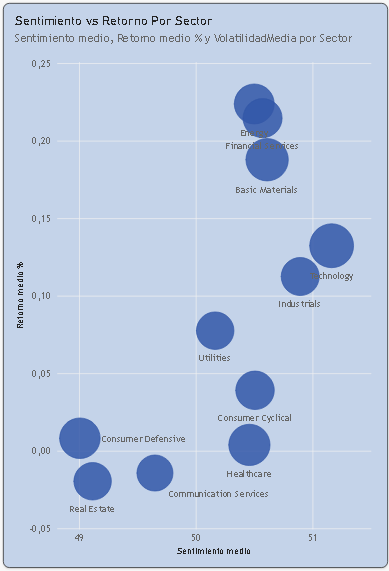
\includegraphics[width=0.55\textwidth]{img/ej6.png}
    \caption{Sentimiento medio frente a retorno medio y volatilidad por sector.}
\end{figure}
\begin{itemize}
    \item \textbf{Gráfico:} diagrama de dispersión y burbujas (\textit{Scatter Chart}), seleccionado según las directrices del enunciado (págs. 8--9) porque permite estudiar de forma simultánea la relación entre dos variables numéricas continuas (\textit{Sentimiento medio} en el eje X y \textit{Retorno medio \%} en el eje Y) agrupadas por sector, incorporando una tercera magnitud en el tamaño de cada punto (\textit{Volatilidad media \%}).
    \item \textbf{Datos y medidas:}
    \begin{itemize}
        \item \textbf{Valores / Categoría:} \code{dim\_sector[Sector]}, representando los 11 sectores del IBEX.
        \item \textbf{Eje X:} \code{hechos[Sentimiento medio]}, el índice de sentimiento asignado por el experto.
        \item \textbf{Eje Y:} \code{hechos[Retorno medio \%]}, el retorno diario porcentual medio de las empresas del sector.
        \item \textbf{Tamaño:} \code{VolatilidadMedia = AVERAGE(hechos[Rango\_Dia\_Pct])}, que refleja la amplitud o volatilidad intradía media.
    \end{itemize}
    Se activan las \textit{Etiquetas de datos} para identificar cada sector de un vistazo en el plano cartesiano.
    \item \textbf{Interacciones:} con \textit{Editar interacciones} se desactiva el filtro procedente del segmentador de \code{Ticker}, garantizando que el gráfico conserve permanentemente la visión global comparativa de todos los sectores del mercado.
    \item \textbf{Análisis de resultados:}
    \begin{itemize}
        \item \textbf{Sentimiento frente a retorno:} los sectores con mayor sentimiento medio (\textit{Technology} con 51,16, \textit{Industrials} con 50,89 y \textit{Financial Services} con 50,57) se sitúan en el cuadrante de rentabilidad positiva más elevada (entre 0,11\,\% y 0,22\,\% diario). Por el contrario, los tres sectores con menor sentimiento medio (\textit{Consumer Defensive} con 49,01, \textit{Real Estate} con 49,12 y \textit{Communication Services} con 49,65) son los únicos que presentan rentabilidades medias negativas o prácticamente nulas ($-0,020\,\%$ en inmobiliario y $-0,014\,\%$ en telecomunicaciones).
        \item \textbf{Riesgo y volatilidad (burbujas):} \textit{Technology} registra la mayor volatilidad media (2,81\,\% de rango intradía) y \textit{Basic Materials} el 2,61\,\%, lo que se traduce en burbujas de mayor diámetro. En el extremo opuesto, \textit{Communication Services} actúa como sector refugio o defensivo con la menor volatilidad del índice (1,84\,\%).
    \end{itemize}
    \item \textbf{Conclusión:} el gráfico valida visualmente que el indicador de sentimiento sectorial de la Práctica 1 muestra consistencia con la evolución bursátil del mercado: sectores con percepción optimista sostenida concentran rentabilidades superiores, mientras que sectores castigados por el sentimiento presentan retornos negativos o planos.
\end{itemize}

\subsection*{Ej7: diseño del dashboard}
\begin{figure}[H]
    \centering
    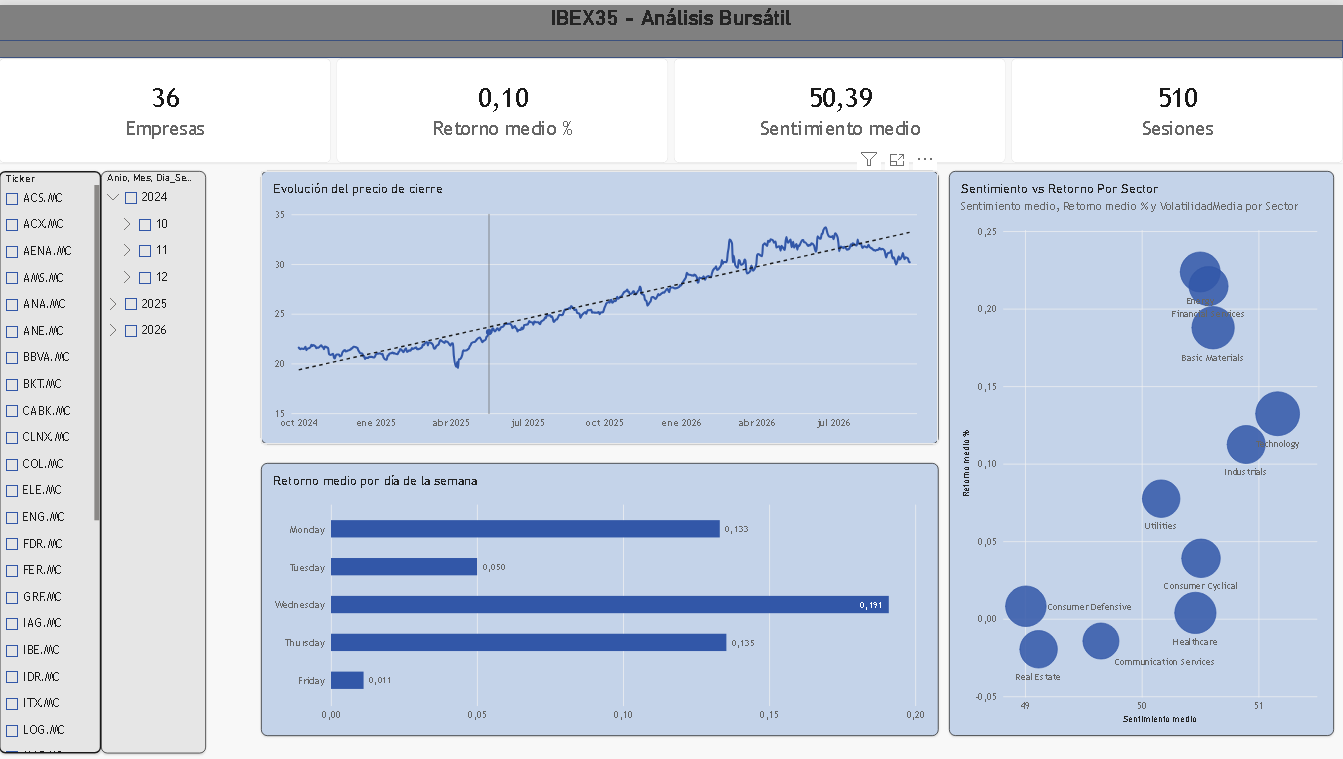
\includegraphics[width=\textwidth]{img/dashboard.png}
    \caption{Vista completa del dashboard final (\textit{IBEX35 - Análisis Bursátil}).}
\end{figure}
\begin{itemize}
    \item \textbf{Público objetivo y propósito del panel:} siguiendo los principios de la guía del enunciado (págs. 7 y 10), el dashboard se orienta a un \textbf{Analista Financiero / Gestor de Carteras} (enfoque analítico-estratégico). Este perfil requiere combinar una visión macro inmediata del mercado (para asignación de activos por sector) con herramientas interactivas de diagnóstico individual (para auditar empresas concretas y contrastar hipótesis cuantitativas como el efecto calendario o la validez predictiva del sentimiento). No es un panel meramente operativo ni para un usuario profano, sino una herramienta de apoyo a la decisión de inversión.
    \item \textbf{Estudio dimensional de variables y relaciones:} para evitar gráficos inconexos y asegurar que cada visualización responda a una pregunta financiera precisa, se definen las relaciones analizadas en la Tabla~\ref{tab:variables_ej7}.
\end{itemize}

\begin{table}[H]
\centering
\small
\begin{tabular}{p{3.5cm}p{3cm}p{2.8cm}p{5.5cm}}
\toprule
\textbf{Variables cruzadas} & \textbf{Visualización} & \textbf{Nivel analítico} & \textbf{Justificación y pregunta de negocio} \\
\midrule
\code{Ticker}, \code{Date}, \code{Sesiones}, \code{Retorno}, \code{Sentimiento} & Tarjetas KPI múltiples (Ej3) & Macro mercado (IBEX) & ¿Cuál es el estado general del mercado? Resume volumen y tono de forma instantánea. \\
\code{Date}, \code{Close} & Líneas con regresión (Ej4) & Temporal continua & ¿Hacia dónde se dirige la acción? Detecta canales de precio, soportes y cambios de ritmo. \\
\code{Dia\_Semana}, \code{Retorno\_Diario\_Pct} & Columnas / Barras (Ej5) & Categórica temporal & ¿Existe estacionalidad semanal? Contrasta empíricamente la hipótesis del efecto viernes. \\
\code{Sentimiento}, \code{Retorno}, \code{Sector}, \code{Volatilidad} & Dispersión y burbujas (Ej6) & Multivariable sectorial & ¿Predice el sentimiento el retorno? Mapea rentabilidad frente a optimismo y riesgo. \\
\bottomrule
\end{tabular}
\caption{Estudio de variables, relaciones y tipos de gráfico elegidos (Ej7).}
\label{tab:variables_ej7}
\end{table}

\begin{itemize}
    \item \textbf{Criterio y orden de lectura (patrón en Z):}
    \begin{enumerate}
        \item \textbf{Cabecera institucional y KPIs (arriba):} banner informativo y tarjeta con cuatro medidas resumen (\textit{Empresas}, \textit{Sesiones}, \textit{Retorno medio \%}, \textit{Sentimiento medio}) para establecer el contexto macro del mercado en un solo golpe de vista.
        \item \textbf{Barra lateral de filtros (izquierda):} segmentadores de \code{Ticker} y fecha (\code{Anio}, \code{Mes}, \code{Dia\_Semana}) colocados a la izquierda para interactuar cómodamente sin desplazar los gráficos.
        \item \textbf{Zona temporal y de empresa (centro):} gráfico de líneas con la evolución diaria del precio de cierre y su recta de regresión, que responde a la selección de una empresa individual.
        \item \textbf{Zona de mercado y contraste de hipótesis (derecha e inferior):} gráfico de barras del efecto día de la semana y gráfico de dispersión de sentimiento frente a retorno por sector, desacoplados del filtro de empresa para mantener la perspectiva transversal del IBEX-35.
    \end{enumerate}
    \item \textbf{Justificación de la distribución:} evita gráficos inconexos y garantiza que cada visual tenga un propósito claro: los KPIs informan del estado global, la línea temporal detalla la empresa analizada y los gráficos de barras y dispersión contrastan hipótesis financieras sobre el conjunto del mercado.
\end{itemize}

\subsection*{Ej8 (opcional): tema}
\begin{itemize}
    \item \textbf{Configuración:} en la pestaña \textit{Vista $\rightarrow$ Temas $\rightarrow$ Personalizar el tema actual} se ha creado un tema corporativo ajustado a estándares de visualización financiera y accesibilidad.
    \item \textbf{Paleta cromática institucional:}
    \begin{itemize}
        \item Azul marino corporativo (\code{\#0F2C59}) como color de énfasis institucional y cabecera.
        \item Verde esmeralda (\code{\#1E8449}) para retornos positivos y variaciones alcistas.
        \item Rojo financiero (\code{\#C0392B}) para rentabilidades negativas y caídas.
        \item Ámbar / Naranja (\code{\#F39C12}) para el índice de sentimiento del experto.
        \item Gris neutro (\code{\#5D6D7E}) para métricas de soporte y volatilidad.
        \item Fondo general en gris claro (\code{\#F8F9F9}) con tarjetas y contenedores en blanco puro (\code{\#FFFFFF}) para maximizar el contraste y evitar la fatiga visual en sesiones prolongadas.
    \end{itemize}
    \item \textbf{Tipografía y jerarquía:} familia \textit{Segoe UI} con tamaños consistentes: títulos de visuales en 12\,pt negrita, valores de tarjetas en 24--28\,pt y etiquetas de datos y ejes en 9--10\,pt con color grafito (\code{\#566573}).
\end{itemize}

\subsection*{Ej9: dashboard por sector}
Se añade la página \textit{Análisis Sectorial} en Power BI para explorar por separado cada uno de los 11 sectores del IBEX. Como se ve en la captura, la página incluye cinco bloques conectados al selector de sector:
\begin{itemize}
    \item \textbf{Selector superior:} botones con la opción \textit{Seleccionar todo} y los 11 sectores (\code{dim\_sector[Sector]}).
    \item \textbf{Precio medio de cierre por empresa (centro izquierda):} gráfico de barras horizontales ordenadas de mayor a menor para comparar qué empresas cotizan a un precio más alto dentro del sector.
    \item \textbf{Retorno medio y sentimiento a lo largo del tiempo (centro derecha):} gráfico temporal (octubre 2024 -- septiembre 2026) que permite ver cómo evolucionan juntos la rentabilidad diaria y el sentimiento del sector.
    \item \textbf{Tabla de empresas (abajo izquierda):} resumen por empresa con su símbolo (\code{Ticker}), nombre, industria, tamaño (\code{MarketCap}), sensibilidad al mercado (\code{Beta}), retorno medio diario y volatilidad media, además de la fila de totales.
    \item \textbf{Tarjetas de resumen (abajo derecha):} cuatro indicadores que se actualizan al elegir un sector (\textit{Retorno medio \%}, \textit{VolatilidadMedia}, \textit{Empresas} y \textit{Sentimiento medio}).
\end{itemize}
En la Tabla~\ref{tab:sectores_resumen} se recogen los valores medios de cada sector en el periodo analizado.

\begin{figure}[H]
    \centering
    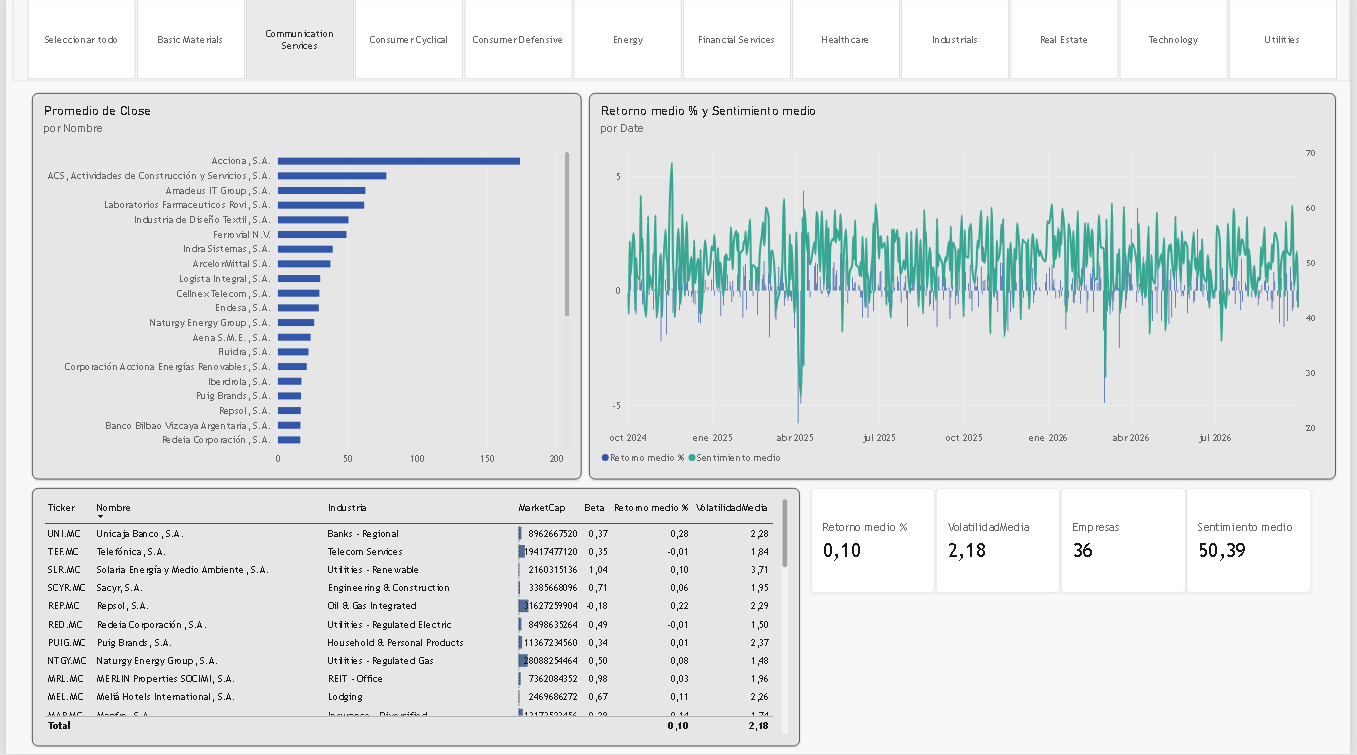
\includegraphics[width=\textwidth]{img/analisis_sectorial.png}
    \caption{Vista de la página \textit{Análisis Sectorial} en Power BI (Ej9).}
\end{figure}

\begin{table}[H]
\centering
\small
\begin{tabular}{lccccc}
\toprule
\textbf{Sector} & \textbf{Empresas} & \textbf{Sentimiento medio} & \textbf{Retorno medio \%} & \textbf{Volatilidad media \%} & \textbf{Beta media} \\
\midrule
Servicios financieros & 7 & 50,57 & +0,215\,\% & 2,19\,\% & 0,44 \\
Industria & 7 & 50,89 & +0,112\,\% & 2,07\,\% & 0,83 \\
Suministros (energía y agua) & 7 & 50,17 & +0,077\,\% & 2,01\,\% & 0,53 \\
Consumo cíclico & 3 & 50,51 & +0,039\,\% & 2,12\,\% & 0,83 \\
Inmobiliario & 3 & 49,12 & $-0,020\,\%$ & 2,00\,\% & 0,72 \\
Materiales básicos & 2 & 50,61 & +0,188\,\% & 2,61\,\% & 1,36 \\
Salud & 2 & 50,46 & +0,004\,\% & 2,46\,\% & 0,72 \\
Tecnología & 2 & 51,16 & +0,132\,\% & 2,81\,\% & 0,82 \\
Comunicaciones & 1 & 49,65 & $-0,014\,\%$ & 1,84\,\% & 0,35 \\
Energía & 1 & 50,50 & +0,224\,\% & 2,29\,\% & $-0,18$ \\
Consumo básico & 1 & 49,01 & +0,008\,\% & 2,37\,\% & 0,34 \\
\bottomrule
\end{tabular}
\caption{Resumen comparativo de métricas por sector (Ej9).}
\label{tab:sectores_resumen}
\end{table}

A continuación se comentan de forma sencilla los resultados de cada sector a partir de los datos del dashboard, viendo tanto las diferencias entre sus empresas como su comportamiento frente al conjunto del IBEX:

\subsubsection*{1. Servicios financieros (7 empresas: Santander, BBVA, CaixaBank, Sabadell, Bankinter, Unicaja, Mapfre)}
\begin{itemize}
    \item \textbf{Dentro del sector:} casi todas las entidades siguen una tendencia parecida y positiva en el periodo, destacando Unicaja (+0,285\,\%), Santander (+0,235\,\%) y BBVA (+0,234\,\%). En cuanto a estabilidad, CaixaBank ($\beta = 0,12$), Bankinter ($\beta = 0,05$) y Mapfre (volatilidad del 1,74\,\%) muestran variaciones más suaves que Santander ($\beta = 0,90$) y BBVA ($\beta = 0,83$), que se mueven más con el mercado.
    \item \textbf{Frente al mercado:} es uno de los sectores con mejor retorno medio del índice (+0,215\,\%) y un sentimiento ligeramente positivo (50,57), mientras que su volatilidad se mantiene en valores intermedios (2,19\,\%).
\end{itemize}

\subsubsection*{2. Industria (7 empresas: Aena, Ferrovial, ACS, IAG, Acciona, Logista, Sacyr)}
\begin{itemize}
    \item \textbf{Dentro del sector:} conviven empresas con precios bastante estables, como Aena (volatilidad del 1,74\,\%) y Ferrovial (1,79\,\%), con otras que tienen subidas y bajadas más marcadas, como la aerolínea IAG (2,71\,\% de volatilidad y $\beta = 1,31$).
    \item \textbf{Frente al mercado:} tiene un comportamiento muy cercano a la media del IBEX, con un retorno diario del +0,112\,\%, una volatilidad moderada (2,07\,\%) y un sentimiento algo optimista (50,89).
\end{itemize}

\subsubsection*{3. Suministros (7 empresas: Iberdrola, Endesa, Naturgy, Redeia, Enagás, Acciona Energía, Solaria)}
\begin{itemize}
    \item \textbf{Dentro del sector:} se aprecia una diferencia clara entre las compañías eléctricas y gasistas tradicionales (Iberdrola, Endesa y Naturgy, con volatilidades bajas de entre 1,48\,\% y 1,66\,\%) y las empresas centradas en renovables, cuyos precios oscilan bastante más (Solaria llega al 3,71\,\% de volatilidad y Acciona Energía al 2,70\,\%).
    \item \textbf{Frente al mercado:} en conjunto es un sector tranquilo (2,01\,\% de volatilidad media), con un sentimiento cercano al punto neutro (50,17) y una rentabilidad positiva moderada (+0,077\,\%).
\end{itemize}

\subsubsection*{4. Tecnología (2 empresas: Amadeus e Indra)}
\begin{itemize}
    \item \textbf{Dentro del sector:} las dos empresas evolucionan de forma muy distinta. Indra registra la mayor subida del periodo (+0,286\,\% de media diaria) acompañada de una volatilidad alta (3,47\,\%), mientras que Amadeus se mantiene prácticamente plana o algo negativa ($-0,021\,\%$) con oscilaciones menores (2,15\,\%).
    \item \textbf{Frente al mercado:} es el sector con el sentimiento medio más alto (51,16) y también el de mayor volatilidad diaria (2,81\,\%), lo que refleja movimientos más intensos que la media del índice.
\end{itemize}

\subsubsection*{5. Materiales básicos (2 empresas: ArcelorMittal y Acerinox)}
\begin{itemize}
    \item \textbf{Dentro del sector:} ambas compañías siderúrgicas suelen moverse en la misma dirección, aunque ArcelorMittal presenta cambios diarios más bruscos ($\beta = 1,71$, la más alta del IBEX, y 2,91\,\% de volatilidad) que Acerinox ($\beta = 1,02$ y 2,30\,\% de volatilidad).
    \item \textbf{Frente al mercado:} combina una rentabilidad media elevada (+0,188\,\%) con una de las volatilidades más altas del índice (2,61\,\%), por lo que sus subidas y bajadas son más pronunciadas que en otros sectores.
\end{itemize}

\subsubsection*{6. Consumo cíclico (3 empresas: Inditex, Fluidra y Meliá Hotels)}
\begin{itemize}
    \item \textbf{Dentro del sector:} Inditex es la empresa de mayor tamaño de todo el IBEX (186\,650 millones de euros) y mantiene una evolución estable (1,92\,\% de volatilidad). Meliá logra el mejor retorno medio del grupo (+0,113\,\%) con algo más de variación diaria (2,26\,\%), mientras que Fluidra termina ligeramente en negativo ($-0,027\,\%$).
    \item \textbf{Frente al mercado:} ofrece resultados discretos en conjunto (+0,039\,\% de retorno medio), con un sentimiento (50,51) y una volatilidad (2,12\,\%) muy próximos a la media general.
\end{itemize}

\subsubsection*{7. Inmobiliario (3 empresas: Merlin Properties, Inmobiliaria Colonial, Inmobiliaria del Sur)}
\begin{itemize}
    \item \textbf{Dentro del sector:} las empresas del grupo comparten una tendencia floja durante estos dos años, sin grandes diferencias entre ellas y con un retorno medio conjunto ligeramente negativo ($-0,020\,\%$).
    \item \textbf{Frente al mercado:} es el sector con peor resultado del periodo, tanto en retorno medio ($-0,020\,\%$) como en sentimiento (49,12), aunque con una volatilidad contenida (2,00\,\%).
\end{itemize}

\subsubsection*{8. Salud (2 empresas: Grifols y Laboratorios Rovi)}
\begin{itemize}
    \item \textbf{Dentro del sector:} las dos empresas muestran caminos opuestos: Grifols tiene mayor inestabilidad en el precio (2,87\,\% de volatilidad, $\beta = 1,26$) y un retorno medio negativo ($-0,033\,\%$), mientras que Rovi logra un resultado positivo (+0,041\,\%) con variaciones más suaves (2,05\,\%, $\beta = 0,18$).
    \item \textbf{Frente al mercado:} al compensarse ambas empresas, la media del sector queda prácticamente neutra en retorno (+0,004\,\%) y con un sentimiento intermedio (50,46).
\end{itemize}

\subsubsection*{9. Comunicaciones (1 empresa: Telefónica)}
\begin{itemize}
    \item \textbf{Dentro del sector:} al haber una única empresa en este grupo (\code{TEF.MC}), los datos del sector coinciden directamente con los de Telefónica.
    \item \textbf{Frente al mercado:} es el valor menos volátil de todo el análisis (1,84\,\% y $\beta = 0,35$), es decir, su precio cambia poco de un día para otro, aunque su retorno medio en el periodo es ligeramente negativo ($-0,014\,\%$) y su sentimiento algo bajo (49,65).
\end{itemize}

\subsubsection*{10. Energía (1 empresa: Repsol)}
\begin{itemize}
    \item \textbf{Dentro del sector:} sector formado únicamente por Repsol (\code{REP.MC}).
    \item \textbf{Frente al mercado:} obtiene el retorno medio diario más alto de todos los sectores (+0,224\,\%). Además, llama la atención su beta negativa ($\beta = -0,18$), lo que indica que en muchos momentos su cotización no sigue la misma dirección que el resto del IBEX.
\end{itemize}

\subsubsection*{11. Consumo básico (1 empresa: Puig Brands)}
\begin{itemize}
    \item \textbf{Dentro del sector:} sector representado únicamente por Puig Brands (\code{PUIG.MC}), incorporada al índice tras empezar a cotizar en mayo de 2024.
    \item \textbf{Frente al mercado:} presenta el sentimiento medio más bajo del listado (49,01) y un retorno medio casi nulo (+0,008\,\%), con algo menos de histórico que el resto de compañías por su reciente incorporación.
\end{itemize}

\end{document}
